\chapter{Device Testing}

This chapter describes the process of testing of the functionality of the device. Testing refers to the robustness of the device itself and testing the functionality of cloning and tag emulation which took place in two layers. In the first layer, the capabilities of Proxmark were tested --- how it can read cards, what information it gives out about the card, how it can detect the keys of different types of Mifare Classic tags and what error messages it gives. This layer builds seamlessly on layer two, which has tested the correctness of the program itself, whether it communicates correctly with Proxmark, and whether it can successfully respond to Proxmark's output, either to notifications of successful operations or to error messages. 


\section{User Notes}

This section presents all the findings and shortcomings that emerged from the testing of the resulting device.

\subsection{Battery Life}
After testing the endurance of the device when powered from a 10,000 mAh power bank, it was found that an idle device, i.e. a switched on Raspberry Pi, with the LCD screen and Proxmark connected, lasts up to 8 hours. This result is very encouraging.

\subsection{Boot Time}
It is essential to mention that one problem starts at boot time. Once the device is plugged into the source, it takes at least about 20 seconds for the device to boot and be usable together with the program created. This is one of the impractical things that has resulted from using this device.

\subsection{Touch Screen}

The use of the touch screen has also shown that it has its shortcomings. Its small refresh rate reduces user-friendliness, and some touches are not detected once in a while. However, these shortcomings do not limit the functionality of the device in any way.

\subsection{Graphical User Interface}
After testing the GUI of the created program, many things were tweaked or corrected.

One of the things that had to be solved was the unpredictable freezing screen when executing a command. This was solved by creating a \texttt{Worker} class that inherits from \texttt{QObject}. This Worker then has the task of managing the created thread that executes the command. The actual implementation can be seen in the code. This method fixes the frozen screen.

Further debugging of the program concerned error messages, so that they are displayed at the right time and disappear appropriately, e.g. when the screen changes.

Another thing that was addressed was making user interaction impossible when a command was in progress --- e.g., disabling buttons.


\section{Tested Tags}
\label{sec:testedtags}

For testing purposes, tags of different types were taken, mostly magic tags. Most of the tags were purchased from China, because of their low price and availability --- there are only a few resellers in our country, who increase the price of these tags. Some of the tags for testing were acquired elsewhere. Here is a list of the specific types of tags that were available for testing the resulting device, most of them are at least two of each, to test cloning, and to be safe, as the tag may get damaged:
\begin{itemize}
    \item Low frequency
    \begin{itemize}
        \item EM410x
        \item EM4x05
    \end{itemize}
    \item High frequency
    \begin{itemize}
        \item Mifare Classic magic tags
        \begin{itemize}
            \item Mifare Classic 1k, 4-byte UID, GEN-2
            \item Mifare Classic 1k, 4-byte UID, GEN-1a/GEN-4
            \item Mifare Classic 4k, 7-byte UID, GEN-3
        \end{itemize}
        \item Mifare Classic non-magic tags
        \begin{itemize}
            \item Mifare Classic 1k, 4-byte UID
            \item Mifare Classic 1k, 7-byte UID
        \end{itemize}
        \item Legic Prime
        \item Mifare Ultralight EV1, non-magic tag
        \item Mifare Ultralight EV1, GEN-2 magic tags
        \item Mifare Desfire, generation 1, 2 or 3
    \end{itemize}
\end{itemize}
Some of these named tags are used for some purpose such as building entrances.

\section{Tag Search Testing}

The program has basic tag identification functions. It can list basic tag information such as UID, magic capabilities or chipset type. This output has been filtered from Proxmark to keep it free of irrelevant information and otherwise more or less preserved. Only 2 scenarios were sufficient to test the functionality, namely when the tag is not near the reader at all --- the program identifies no tag found, and the case when the tag is successfully read. These two scenarios were tested for both LF and HF tags separately.

\section{Tags Cloning Testing}
Testing of tag cloning was done separately for each tag type. It should be noted that tag cloning means transferring the data content of one tag to another while preserving the original manufacturer data --- i.e., for example, the tag UID. Changing the UID is tested later in this chapter.

\subsection{Mifare Classic}
\label{subsec:mifareclassiccloning}

Cloning Mifare Classic tags is one of the most complex cloning used in this work, but still quite straightforward. 

First, it was tested if Proxmark could retrieve the keys of all the tested Mifare Classic tags. With only slight difficulties, all keys were obtained --- even the keys of the non-magic tags. Difficulties encountered can only be attributed to the quality of the data transfer between the reader and the tag. Sometimes other tags near the reader interfered with the communication, sometimes it was enough to move the tag to a better position on the HF tag reader.

Testing was carried out on the available Mifare Classic magic tags and the two classic Mifare Classic tags that are used in real-world applications, for example entrance tags. One of the tags is used to enter an unnamed gym. Reading and searching for keys is done a little differently on each tag, depending on which Mifare Classic vulnerability Proxmark is currently exploiting. Most of the keys were read in about 20 seconds, with one exception which was read in about 60 seconds.

With all the keys retrieved, the tag dumps were also saved. In order to write this data to another tag, the keys of the destination tag must also be saved. Only then can the Mifare Classic tag be written.

Writing all sectors to a Mifare Classic 1k tag takes around 15 seconds, while writing to a Mifare Classic 4k tag sometimes takes up to one minute. The process of cloning this type of tag is the most complicated, also because of the duration.

Therefore, when testing Mifare Classic, I did not come into contact with a tag whose keys could not be obtained in this way. In these cases, the resulting device, in its current state, would not be able to clone the Mifare Classic cards. Verification that the write to the target tag was successful was done by comparing the dumpfiles.

\subsubsection{Real-World Example}
The keys of the aforementioned tag used to enter the gym were successfully retrieved by the device and so were the contents of the card. Unfortunately, this card has a 7 byte UID and is of Mifare Classic 1k type and the only available 7 byte magic tag was Mifare Classic 4k type, the other magic tags only had 4 byte UIDs. However, thanks to backwards compatibility, it was possible to copy the contents of the original tag into the first part of the memory and change the UID accordingly. As a result, there was a tag with the same UID and the same data blocks in sectors 0 to 15. After trying to access the gym with the newly cloned tag, it was found that the access was granted and the system therefore did not check the size of the Mifare Classic.

\subsection{Mifare Ultralight}

Unlike the Mifare Classic, the Mifare Ultralight tag is very straightforward to read. When the device is reading the simplest type of Mifare Ultralight, it reads all pages. However, when the type is Mifare Ultralight EV1, the device reads only the unprotected pages, see Chapter~\ref{chap:theory}. This was verified by testing the reading of Ultralight tags. In a moment the card is read, the data dump is ready to move to another tag. Writing to the target tag went always smoothly, the success of the operation was verified by reading the contents of the written tag. 

\subsection{Legic Prime}

Unfortunately, the cloning of the Legic Prime tag has not been tested as it should. Since there was only one tag available, it was only possible to read that tag and write the same tag again. In this respect, it relied on the software in Proxmark, where it was only possible to determine the success rate of writing to that one tag and not to any other.


\section{Tags Emulating Testing}

The testing of tag emulation was of course limited because the number of different readers is limited. The readers that were available were only those that I had already used myself to enter buildings or for identification, and thus no unauthorized access was gained in any case. Additionally, another Proxmark helped with testing the emulation, which always read what the device was emulating. The emulated data could be used to determine the success rate.

\subsection{Two Types of Emulation}
\label{subsec:twotypes}

If the user is unable to get the entire content of the tag, the Proxmark software allows emulation only of the UID (and its associated manufacturer data) of these types of tags:

\begin{itemize}
    \item EM410x,
    \item Mifare Classic,
    \item Mifare DESFire, and
    \item Mifare Ultralight.
\end{itemize}
The device therefore pretends to the reader as the tag type with the set UID. Of course, any additional data in the tag is incorrect and irrelevant.

Of course, many systems require the tag to contain other inaccessible data that is considered secure. In order to emulate these tags, the device must first successfully read the contents of the tag and, in the case of Mifare Classic, its keys. In this paper, the focus is on emulating the data content of these types of tags:

\begin{itemize}
    \item Mifare Classic,
    \item Mifare Ultralight, and
    \item Legic Prime.
\end{itemize}

\subsection{EM410x}

When trying to emulate EM410x tags, there was a problem that the readers could not detect the emulation. A bug in the developed software can be ruled out thanks to the logs generated by the program. It can therefore be attributed to either the Proxmark3 software controlling Proxmark 3 Easy or it may be a hardware problem. A hardware problem is more likely, as after reviewing the Proxmark community posts, people were experiencing a similar problem, and for some the emulation worked without issue~\cite{notworkingemulation}.

After reviewing the emulation and trying to load the emulated tag with a second Proxmark, the problem was confirmed, namely that the Proxmark does not emulate the tag type EM410x at all. If the above reasoning is correct, this could be fixed by replacing the Proxmark 3 Easy with another unit in which the hardware problem does not occur. However, when the Proxmark of the resulting device was replaced with the second one, the emulation was also unsuccessful. Therefore, it is possible that both of the tested Proxmarks have this defect, but another error cannot be ruled out as well.


\subsection{Mifare Classic}
As mentioned in Subsection~\ref{subsec:twotypes}, the Proxmark software supports emulation of either the UID itself or emulation of the entire tag including sectors. For Mifare Classic, Proxmark supports emulation of the UID only for the types Mifare Classic 1k, Mifare Classic 4k. Emulation of only the UID was successful --- the output of the second Proxmark, that read the emulated data can be seen in Figure~\ref{fig:emulateduidclassic}

\begin{figure}[ht]
  \centering
  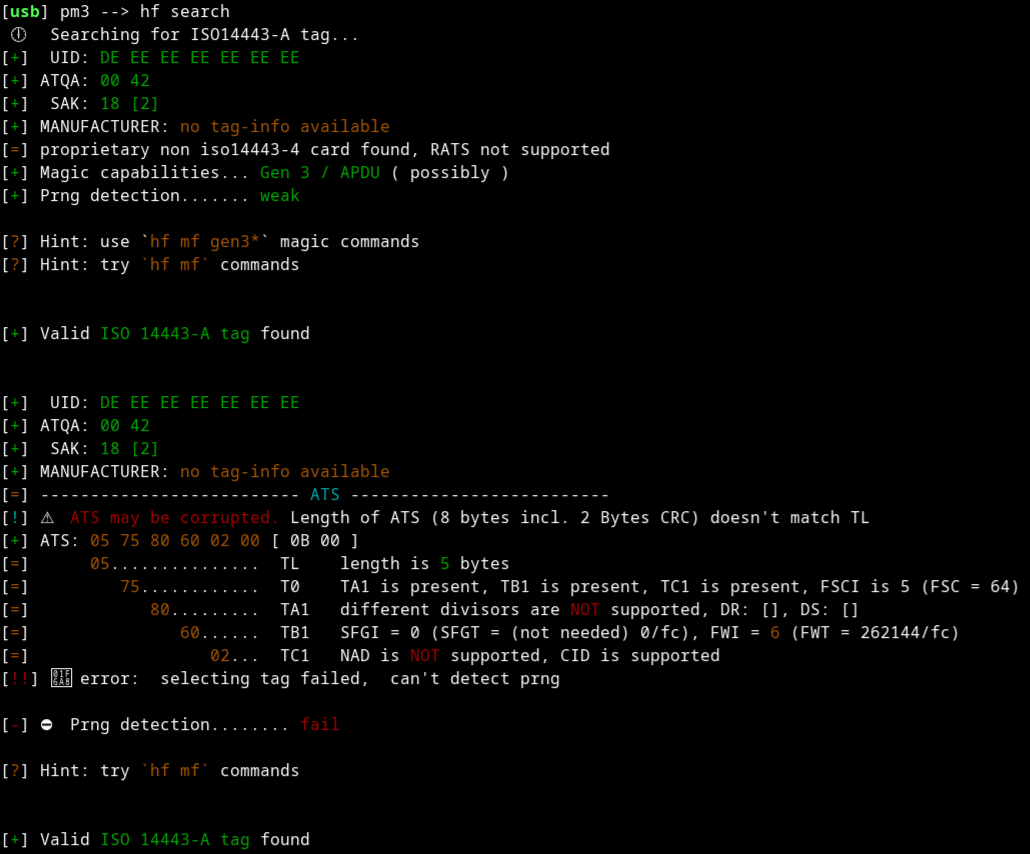
\includegraphics[width=12cm]{text/testing/classic_4k_uid.png}
  \caption{~Output of the second Proxmark when reading the emulated UID of Mifare Classic 4k.}
  \label{fig:emulateduidclassic}
\end{figure}

Emulation of all sectors of the tag is supported by Proxmark for types

\begin{itemize}
    \item Mifare Classic 1k,
    \item Mifare Classic 4k,
    \item Mifare Classic 2k,
    \item Mifare Classic Mini.
\end{itemize}

For proper emulation it was first necessary to read a Mifare Classic tag and save a dump of its memory. Testing the reading and cracking of Mifare Classic is described in Subsection~\ref{subsec:mifareclassiccloning}. The emulation was tested with another Proxmark that read the emulated tag to verify correctness. A photo of this process can be seen in Figure~\ref{fig:proxmarkemulatingtesting} and a screenshot of how the second Proxmark read the emulated data can be seen in Figure~\ref{fig:emulatedblocksclassic}.

\begin{figure}[ht]
  \centering
  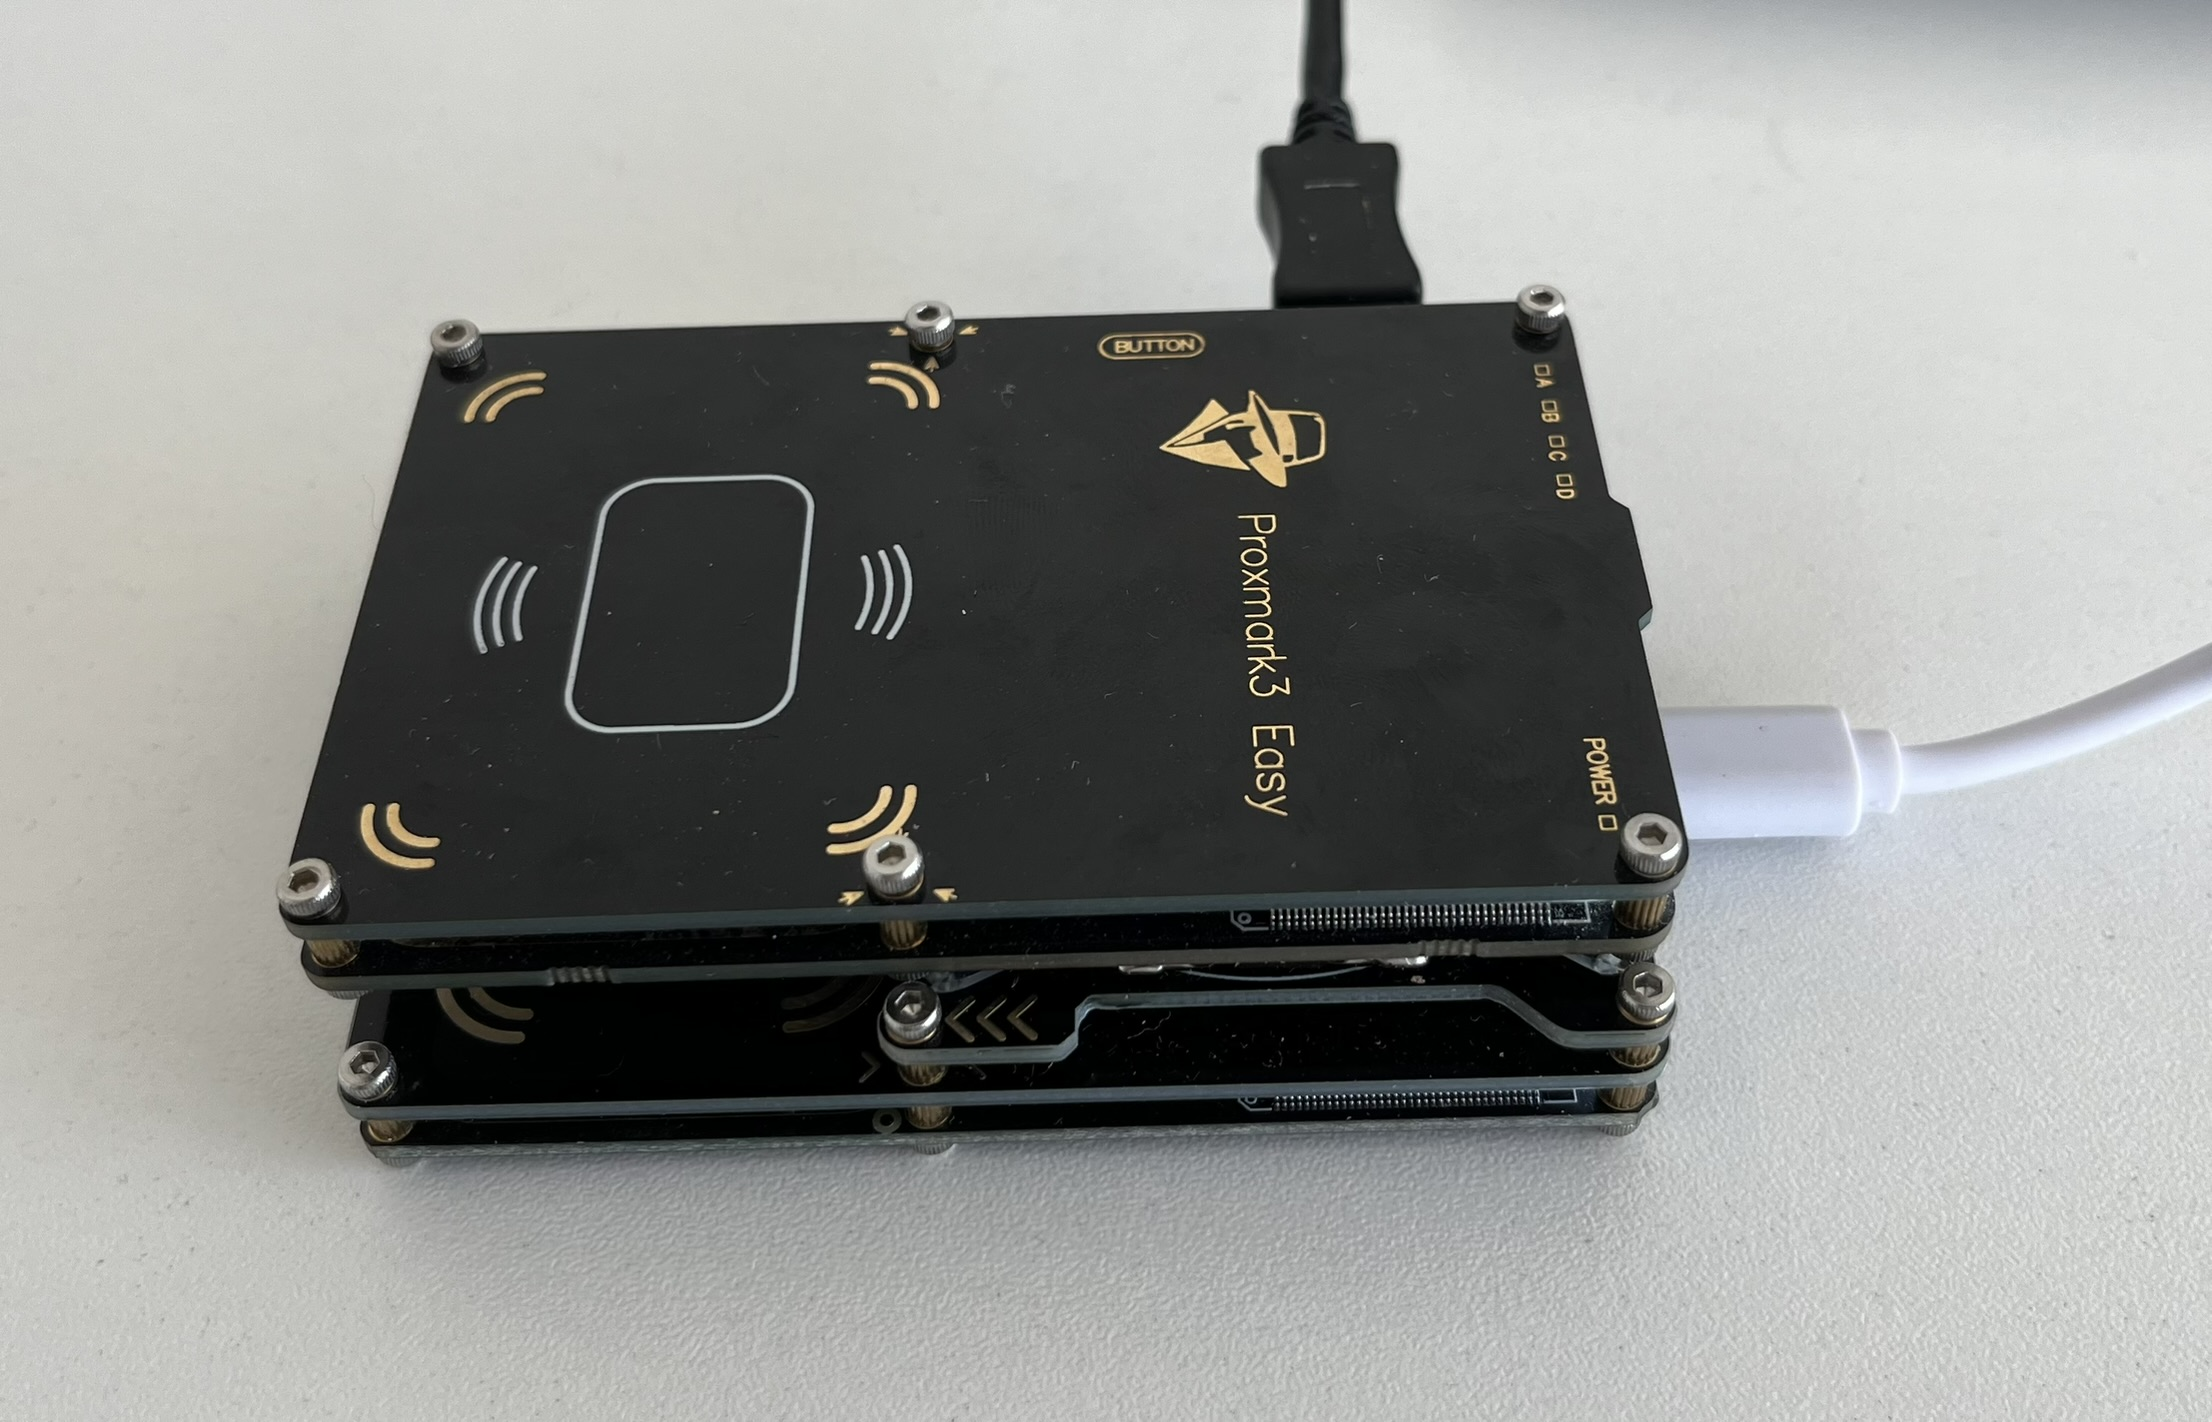
\includegraphics[width=7cm]{text/testing/two_proxmarks.JPEG}
  \caption{~Two Proxmarks on top of each other --- emulation testing.}
  \label{fig:proxmarkemulatingtesting}
\end{figure}

\begin{figure}[ht]
  \centering
  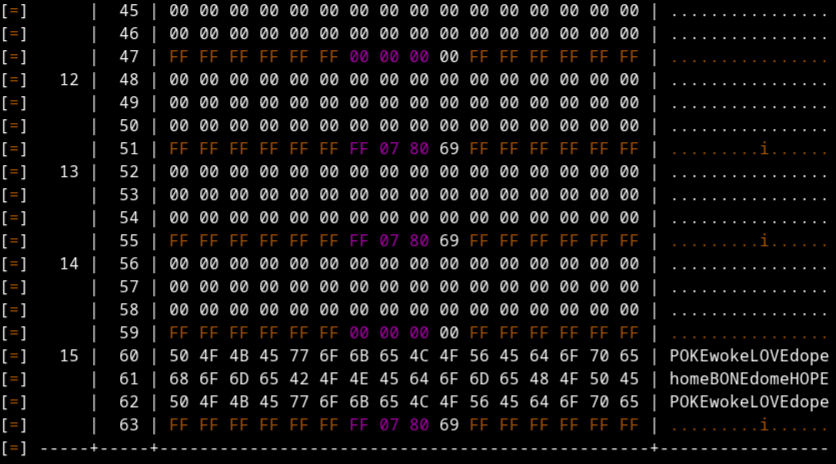
\includegraphics[width=9cm]{text/testing/whole_mf_classic_4k.png}
  \caption{~Reading emulated blocks of Mifare Classic 1k.}
  \label{fig:emulatedblocksclassic}
\end{figure}

Unfortunately, I did not have the opportunity to test the emulation of the Mifare Classic tag in a working system, e.g. the emulation of the tag used to enter the gym, which I managed to clone, see Subsection~\ref{subsec:mifareclassiccloning}.

\subsection{Mifare Ultralight}

Mifare Ultralight tags can be emulated by Proxmark --- pages that have been read. There is again the possibility of emulating just the UID with undefined data pages. Both were tested with a second Proxmark, where a problem was identified. The Proxmark correctly emulated the entered UID of the tag, however, the ATQA and SAK values were wrong. The original Mifare Ultralight tag has ATQA value \texttt{0044} and SAK \texttt{00}. As seen in Figure~\ref{fig:emulatedidultralight}, the device emulated a tag with ATQA value \texttt{0344} and SAK \texttt{00}.

\begin{figure}[ht]
  \centering
  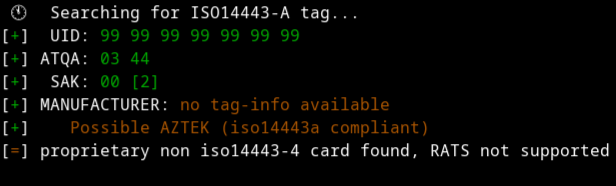
\includegraphics[width=9cm]{text/testing/id_ultralight_wrong _atqa.png}
  \caption{~Wrong ATQA value while emulating Mifare Ultralight.}
  \label{fig:emulatedidultralight}
\end{figure}

After loading a whole Mifare Ultralight tag into emulator's memory, another problem arose. It was not possible to read the blocks of data of the emulated tag. Unfortunately, I did not come into contact with a real-world use of the Mifare Ultralight tag during the testing, so I do not provide a real-world example. It is not a significant drawback that the emulation of Mifare Ultralight does not work as expected, as there was no problem with Mifare Ultralight cloning.

\subsection{Mifare Desfire}
For Mifare DESfire type tags, Proxmark allows emulation of the tag UID only, and this is of course because the card is not known to be attacked and is considered secure~\cite{preucil2023surveying}. 

Testing was therefore conducted again with the second Proxmark as the reader that could read the UID correctly with appropriate ATQA, SAK and ATS values, see Figure~\ref{fig:desfireemulation}.

\begin{figure}[ht]
  \centering
  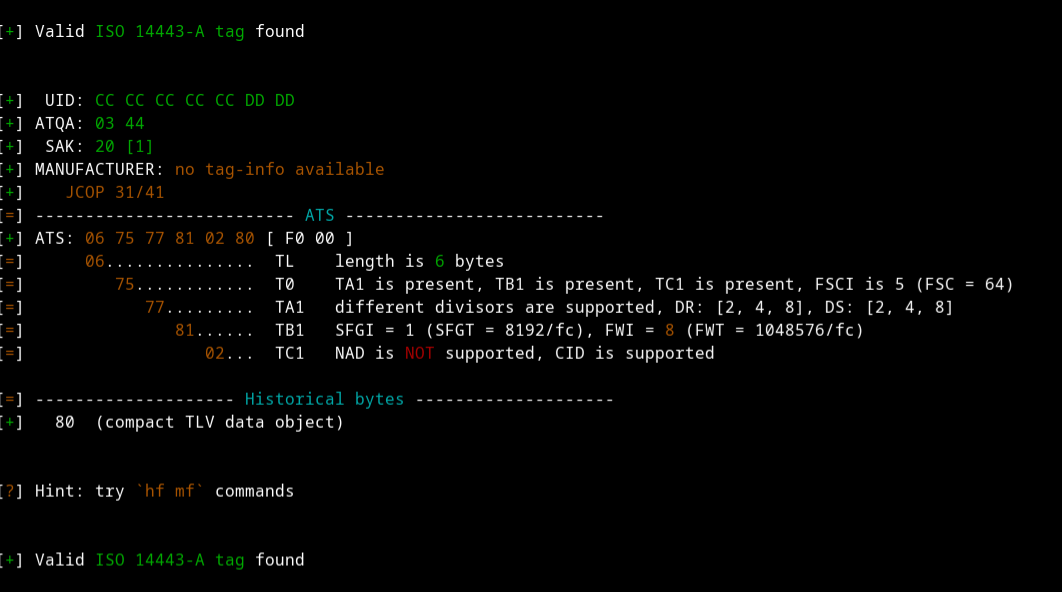
\includegraphics[width=13cm]{text/testing/des_emulation.png}
  \caption{~Emulated Mifare DESFire, read by second Proxmark.}
  \label{fig:desfireemulation}
\end{figure}

\subsubsection{Real-World Example}
To test the Mifare DESfire tag emulation, I had two tags used to access an unnamed organization and an unnamed school building --- this tag is used, among other things, to pay for lunches in the school cafeteria and to enter the dormitory. 

For the unnamed organization, simply emulating the 7 byte UID DESFire tag was not enough --- access to the building was not granted. Conversely, for the unnamed school's building entrance, emulation of the UID tag alone passed, for the main entrance and for entrances to individual classrooms within the building, even for entry to the dorm areas. Payment using the emulated tag in the student cafeteria was not tested.

For testing, a given 7 byte UID of the school DESFire tag was written to a 7 byte Mifare Classic 4k tag. With this newly created Mifare Classic tag, access was only granted in the school building and not in the dormitory areas. This is because some of the readers are also checking the type of the tag --- ATQA and SAK values, which were in this case different. However, they were correctly emulated by the device before, that explains the granted access to the emulated DESFire tag.

\subsection{Legic Prime}

The Legic Prime tag emulation was tested again using another Proxmark, which successfully read the emulated Legic Prime tag. A photo from the process can be seen in Figure~\ref{fig:legicemulation}. However, the testing was very limited by the number of available Legic Prime tags. 

\begin{figure}[ht]
  \centering
  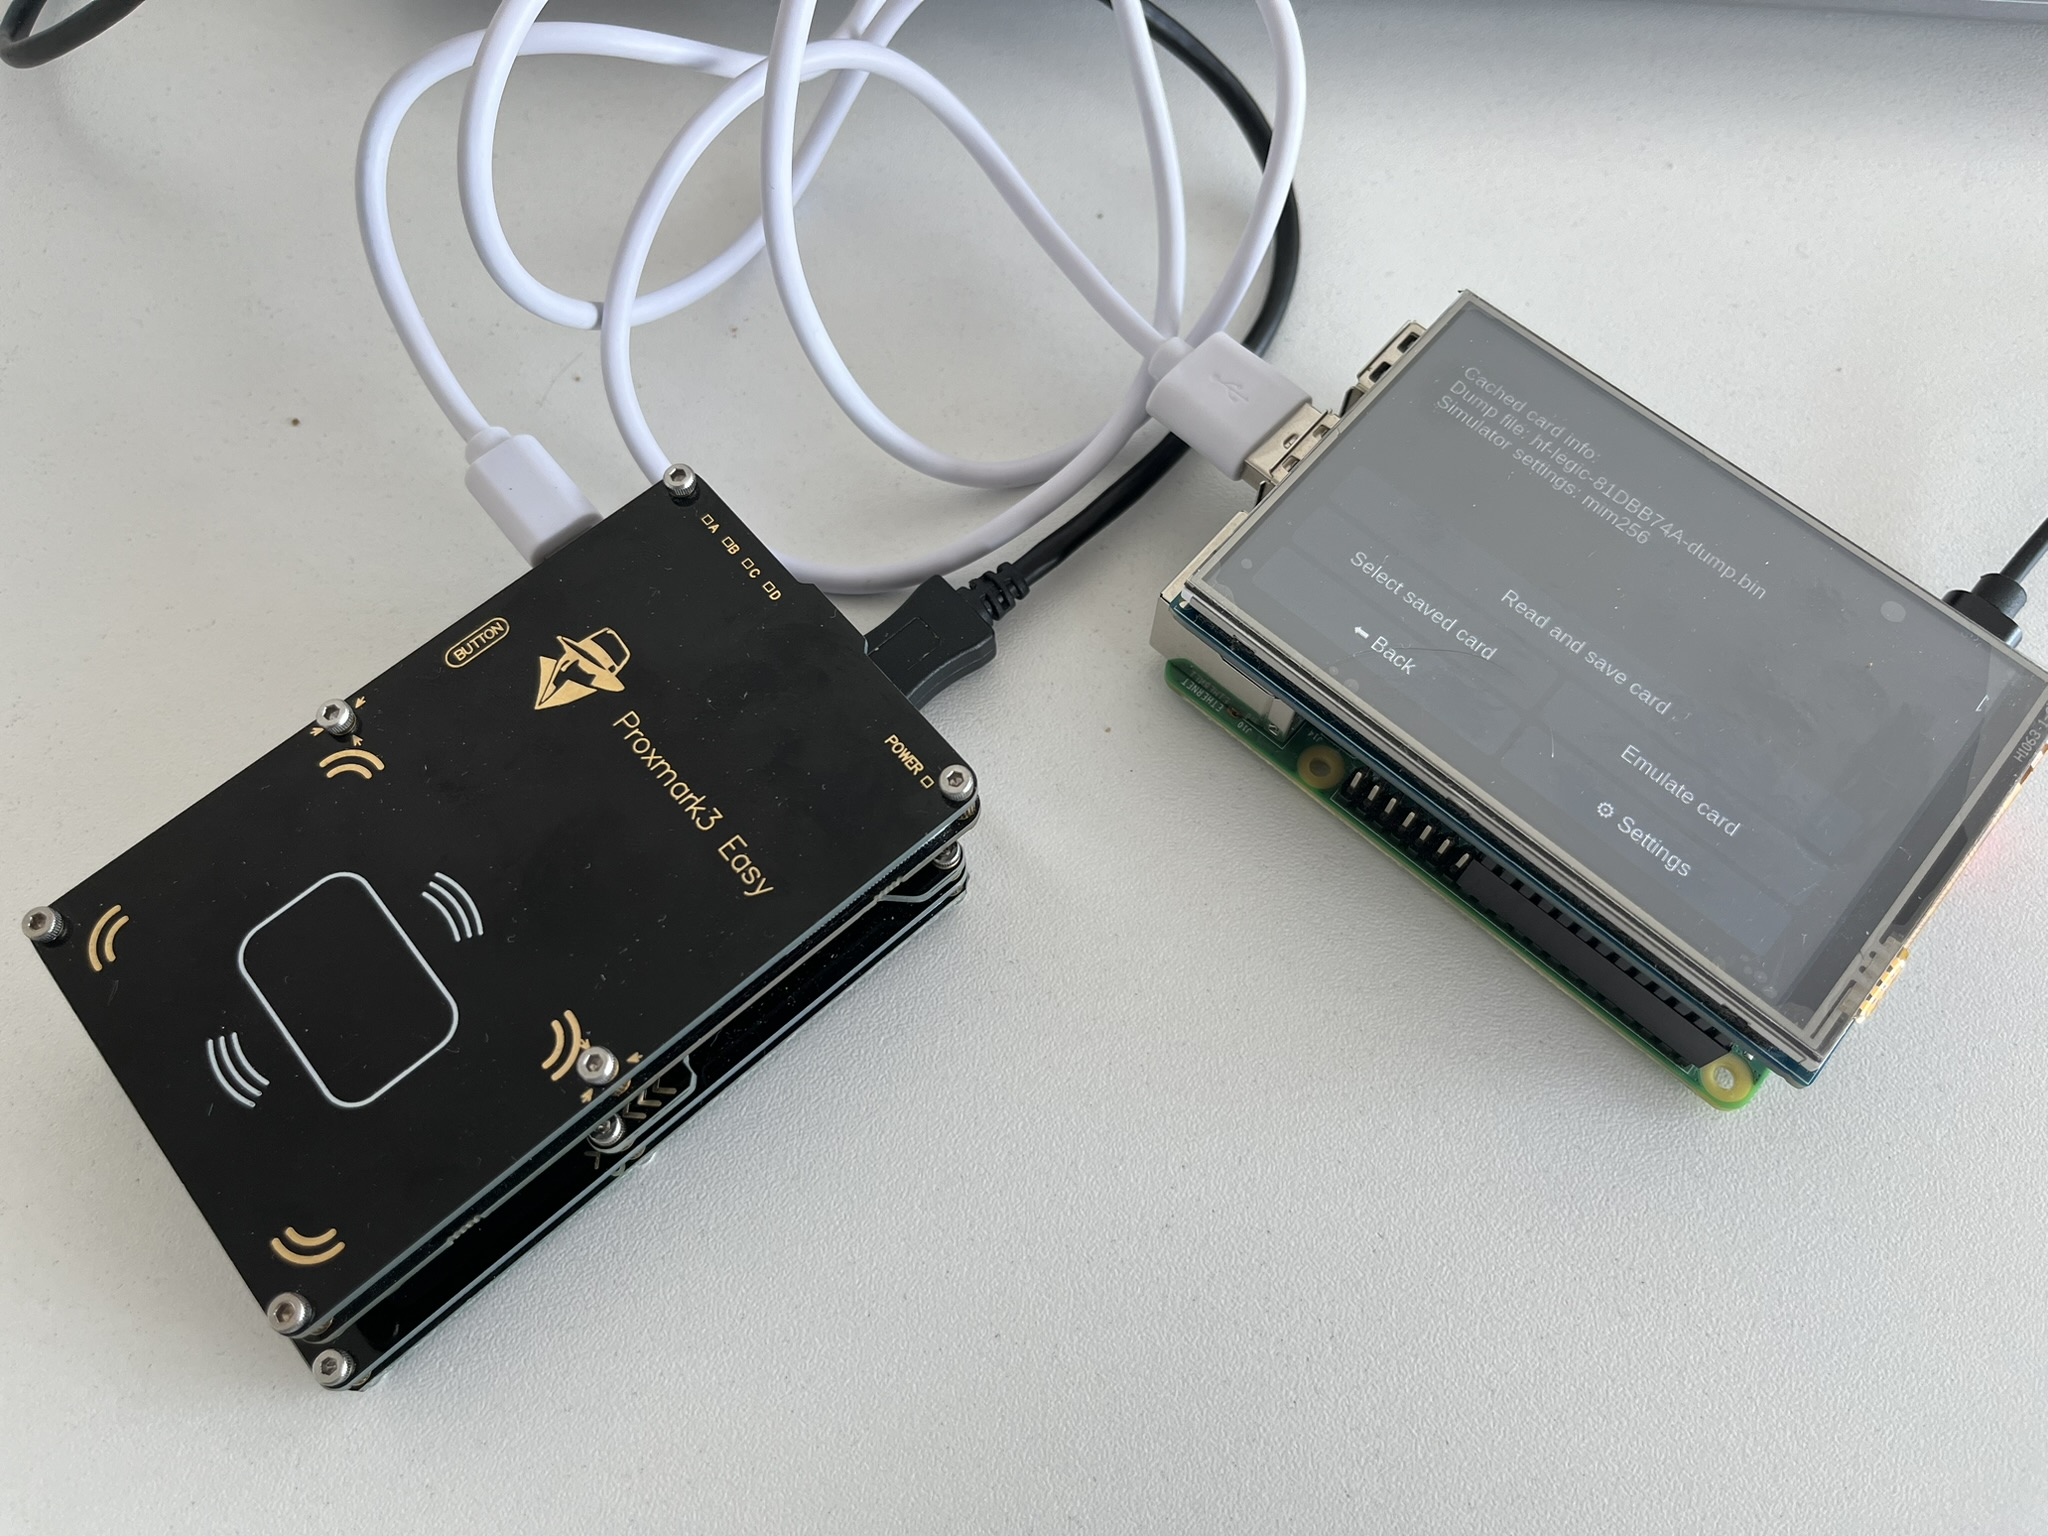
\includegraphics[width=10cm]{text/testing/emulating_legic.JPEG}
  \caption{~Emulating Legic Prime tag.}
  \label{fig:legicemulation}
\end{figure}


\section{UID Changing Testing}
Generally speaking, changing the UID of magic tags went smoothly, but it always needs to be considered e.g. which generation of magic tag it is, because these tags are controlled by different commands. A couple of times it happened that the tag was broken in response to the wrong command.

\subsection{EM410x}
Exactly with that tag, it depended on the chipset inside. If the tag UID was changed with the T5577 chipset but the encoding for Q5/T5555 was used, the tag was broken. The tag could be fixed by changing the UID and using the correct encoding.

Otherwise, changing the UID of these tags was very straightforward and there were no problems, which is due to the simple tag architecture.

\subsubsection{Real-World Example}
Since there were a lot of EM410x type LF tags available, both the magic ones that can change the UID, but also the ones that are already in use for some operational purposes, such as building entrances or identification in an unnamed canteen, testing the change of the UID was very straightforward and simple. The device was able to change UID of every given magic tag of type EM410x. Thus, the readers in the given buildings read the content of the magic tags without any problem, granting access for those that had the UID of the original tag. 

\subsection{Mifare Classic}
As seen in section~\ref{sec:testedtags}, there were several types of magic Mifare Classic tags available. Each is controlled by different commands and thus there is a distinction between the different types in the device. Therefore, when changing the UID of a magic Mifare Classic tag, it is first necessary to find out what generation it is. This can be easily determined by an HF search, which will give out important information about the tag. Then the appropriate generation needs to be set in the settings. Changing the UID then goes smoothly, during multiple testing of all available tags no problems arose, except when the generation of the magic tag was set incorrectly. Verification of the UID change was done simply by reloading the tag with the device.


\subsection{Mifare Ultralight}
When testing the Mifare Ultralight tag UID change, there was only a minor issue with one of the three tags. The tag had to be positioned perfectly on the reader for the UID change to succeed. The other two tags had no problem with this. After the UID change, the operation was verified by reloading the tag.
